\documentclass[man,floatsintext]{apa6}
\usepackage[nodoi]{apacite}
\usepackage{graphicx}
\usepackage{amsmath}
\usepackage[american]{babel}
\usepackage[section]{placeins}

\title{An Integrative Account of Constraints on Cross-Situational Learning}
\author{Daniel Yurovsky and Michael C. Frank}
\affiliation{Department of Psychology, Stanford University}
\shorttitle{Integrating Cross-Situational Learning}
\leftheader{Yurovsky \& Frank}

\abstract{Word-object co-occurrence statistics are a powerful information source for vocabulary learning, but there is considerable debate about how learners actually use them. While some theories hold that learners accumulate graded, statistical evidence about multiple referents for each word, others suggest that they track only a single candidate referent. In two large-scale experiments, we show that neither account is sufficient: Cross-situational learning involves elements of both. Further, the empirical data are captured by a computational model that formalizes how memory and attention interact with co-occurrence tracking. Together, the data and model unify opposing positions in a complex debate and underscore the value of understanding the interaction between computational and algorithmic levels of explanation.}

\keywords{statistical learning, word learning, language acquisition, computational models}
\authornote{We are grateful to Linda Smith, Elika Bergelson, Molly Lewis, Ann Nordmeyer, and all of the members of the Language and Cognition Lab for their feedback on this project. This work was supported by a NIH NRSA F32HD075577 to DY and a grant from the Merck Scholars Foundation to MCF. 

\vspace{12pt}

Please address correspondence to Daniel Yurovsky, Jordan Hall (Building 420), Stanford University, 450 Serra Mall, Stanford, CA 94305. Email: yurovsky@stanford.edu}

\begin{document}
\maketitle

Natural languages are richly structured. From sounds to phonemes to words to referents in the world, statistical regularities characterize the units and their connections at every level. Adults, children, and even infants have been shown to be sensitive to these statistics, leading to a view of language acquisition as a parallel, possibly implicit, process of statistical extraction \cite{Saffran1996a, Gomez2000}. Recent experiments across a number of domains, however, show that human statistical learning may be significantly more limited than previously believed \cite{Johnson2010c, Yurovsky2012c, Trueswell2013}.

We focus here on the use of statistical regularities to learning the meanings of concrete nouns (known as cross-situational word learning; \citeNP{Pinker1989, Siskind1996, Yu2007}). Because words' meanings are reflected in the statistics of their use across contexts, learners could discover the meaning of the word ``ball'' (for instance) by noticing that while it is heard across many ambiguous contexts, it often accompanies play with small, round toys. A growing body of experiments shows that adults, children, and infants are sensitive to such co-occurrence information, and can use it to map words to their referents \cite{Yu2007, Smith2008, Vlach2013, Suanda2014}.

Information about a word's meaning can thus be extracted from the environmental statistics of its use \cite{Siskind1996,Frank2009a}. But this analysis is posed at what \citeA{Marr1982} called the ``computational theory'' level: dealing only with the nature of the information available to the learner. At the ``algorithmic'' level---the level of psychological instantiation in the mind of the learner---this idealized statistical computation could be realized in many ways, and the computation human learners actually perform is a topic of significant debate \cite<see e.g.,>{Yu2012b}. 

Do human learners really maintain a representation of word-object co-occurrences? Some evidence suggests that humans are indeed gradual, parallel accumulators of statistical regularities about the entire system of word-object co-occurrences, simultaneously acquiring information about multiple candidate referents for the same word \cite{Vouloumanos2008, McMurray2012, Yurovsky2014}. Other evidence suggests that statistical learning is a focused, discrete process in which learners maintain a single hypothesis about the referent of any given word. This referent is either verified by future consistent co-occurrences or instead rejected, ``resetting'' the learning process \cite{Medina2011, Trueswell2013}. While both of these algorithmic-level solutions will, in the limit, produce successful word-referent mapping, they will do so at very different rates. In particular, if learners track a only a single referent for each word, it may be necessary to posit additional biases and constraints on learners in order for human-scale lexicons to be learned in human-scale time from the input available to children \cite{Blythe2010,Reisenauer2013}.

To distinguish between these two accounts, previous experiments exposed learners to words and objects in which co-occurrence frequencies indicated several high-probability referents for the same word. At the group level, participants in these experiments showed gradual learning of multiple referents for the same word \cite<e.g.,>{Vouloumanos2008, Yurovsky2013}; but gradual, parallel learning curves can be observed at the group level even if individuals are discrete, single-referent learners \cite{Gallistel2004, Medina2011}. Experiments measuring the same learner at multiple points---a stronger test---have produced mixed results. In some cases, learners showed clear evidence of tracking multiple referents for each word, suggesting a distributional approximation mechanism at the algorithmic level \cite{Smith2011a, Yurovsky2013a, Dautriche2014}. In other experiments, however, learners appear to track only a single candidate referent, and to restart from scratch if their best guess is wrong \cite{Medina2011, Trueswell2013}. 

\vspace{24 pt}

 \begin{figure}[tb]
	\center{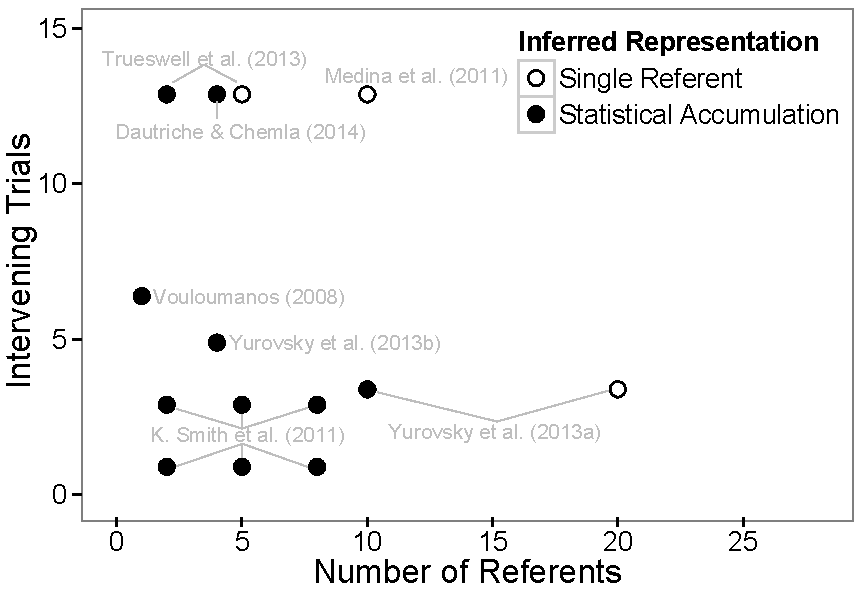
\includegraphics[width=.8\textwidth]{figures/multiple_refs}}
	\caption{\label{fig:mrefs} Results of previous experiments investigating representations for cross-situational learning. These experiments vary along a number of dimensions, but two appear to predict whether multiple-referent tracking is observed: the number of referents present on each trial, and the interval between trials for the referent.}
\end{figure}

These mixed results expose a fundamental gap in our understanding of the mechanisms humans use to encode and track environmental statistics critical for learning language. Evidence for each account is separately compelling, but neither account can explain the evidence used to support the other. Because previous experiments differ along a number of dimensions---e.g., methodology, stimuli, timing, and precision of measurement---it has been difficult to integrate them to understand why cross-situational learning sometimes appear distributional and sometimes appear discrete \cite<for a review, see>{Yurovsky2014}. 

We propose that differences in task difficulty may explain diverging results across experiments. Two salient dimensions vary across previous studies: ambiguity of individual learning instances, and the interval between successive exposures to the same label (Fig.~\ref{fig:mrefs}). As attentional and memory demands increase, learners may shift from statistical accumulation to single-referent tracking \cite{Smith2011a, Trueswell2013}. 

We present a test of this hypothesis, adapting a paradigm first introduced in \citeA{Bower1963} to study the information learners store in concept identification. We parametrically manipulated both the ambiguity of individual learning trials and the interval between them and measured multiple-referent tracking at the individual-participant level. Even at the maximum difficulty tested, learners tracked multiple referents for each word; this result constitutes strong evidence against a qualitative shift from statistical accumulation to single-referent tracking. The data also show that learners encode the referents with differing strengths, however, remembering their hypothesized referent much better. Thus, each previous account appears to be partially correct. 

To clarify how these two accounts are related, we implemented both single-referent tracking and statistical accumulation as computational models. We also extended these accounts into an integrative model that subsumes both as special cases along a continuum. Only the integrative model accounted for our full dataset. Further, this model was able to make nearly perfect parameter-free predictions for a follow-up experiment that was designed to verify that learners encode mappings rather than individual words and objects. We conclude that cross-situational word learning is best characterized by an integrative account: Learners track both a single target referent and an approximation to the co-occurrence statistics; the strength of this approximation varies with the complexity of the learning environment.

\section{Experiment 1}

We designed Experiment 1 to estimate learners' memory for both their single best hypothesis about the correct referent of a novel word and their additional statistical knowledge as demands on attention and memory varied. Participants saw a series of individually ambiguous word learning trials in which they heard one novel word, viewed multiple novel objects, and made guesses about which object went with each word. To succeed, participants needed to encode at least one of the objects that co-occurred with a word, remember it until their next encounter with that word, and check whether that same object was again present. If participants encoded exactly one object, they would succeed only when their initial hypothesis was correct. However, the more \emph{additional} objects participants encoded on their first encounter with a word, the greater their likelihood of succeeding even if their initial hypothesis was incorrect. 

Rather than allowing chance to determine whether participants held the correct hypothesis on their first exposure to a novel word, the set of novel objects presented on the second exposure to each word was constructed based on participants' choices. On \emph{Same} trials, the participant's hypothesized referent was pitted against a set of novel competitors. In contrast, on \emph{Switch} trials, one of the objects the participant had previously \emph{not} hypothesized was pitted against a set of novel competitors (see Fig.~\ref{fig:design}). Logically, either a single-referent tracking or a statistical accumulation mechanism will succeed on Same trials. However, only statistical accumulation of information about non-target items can  succeed on Switch trials.

\begin{figure}[tb]
	\center{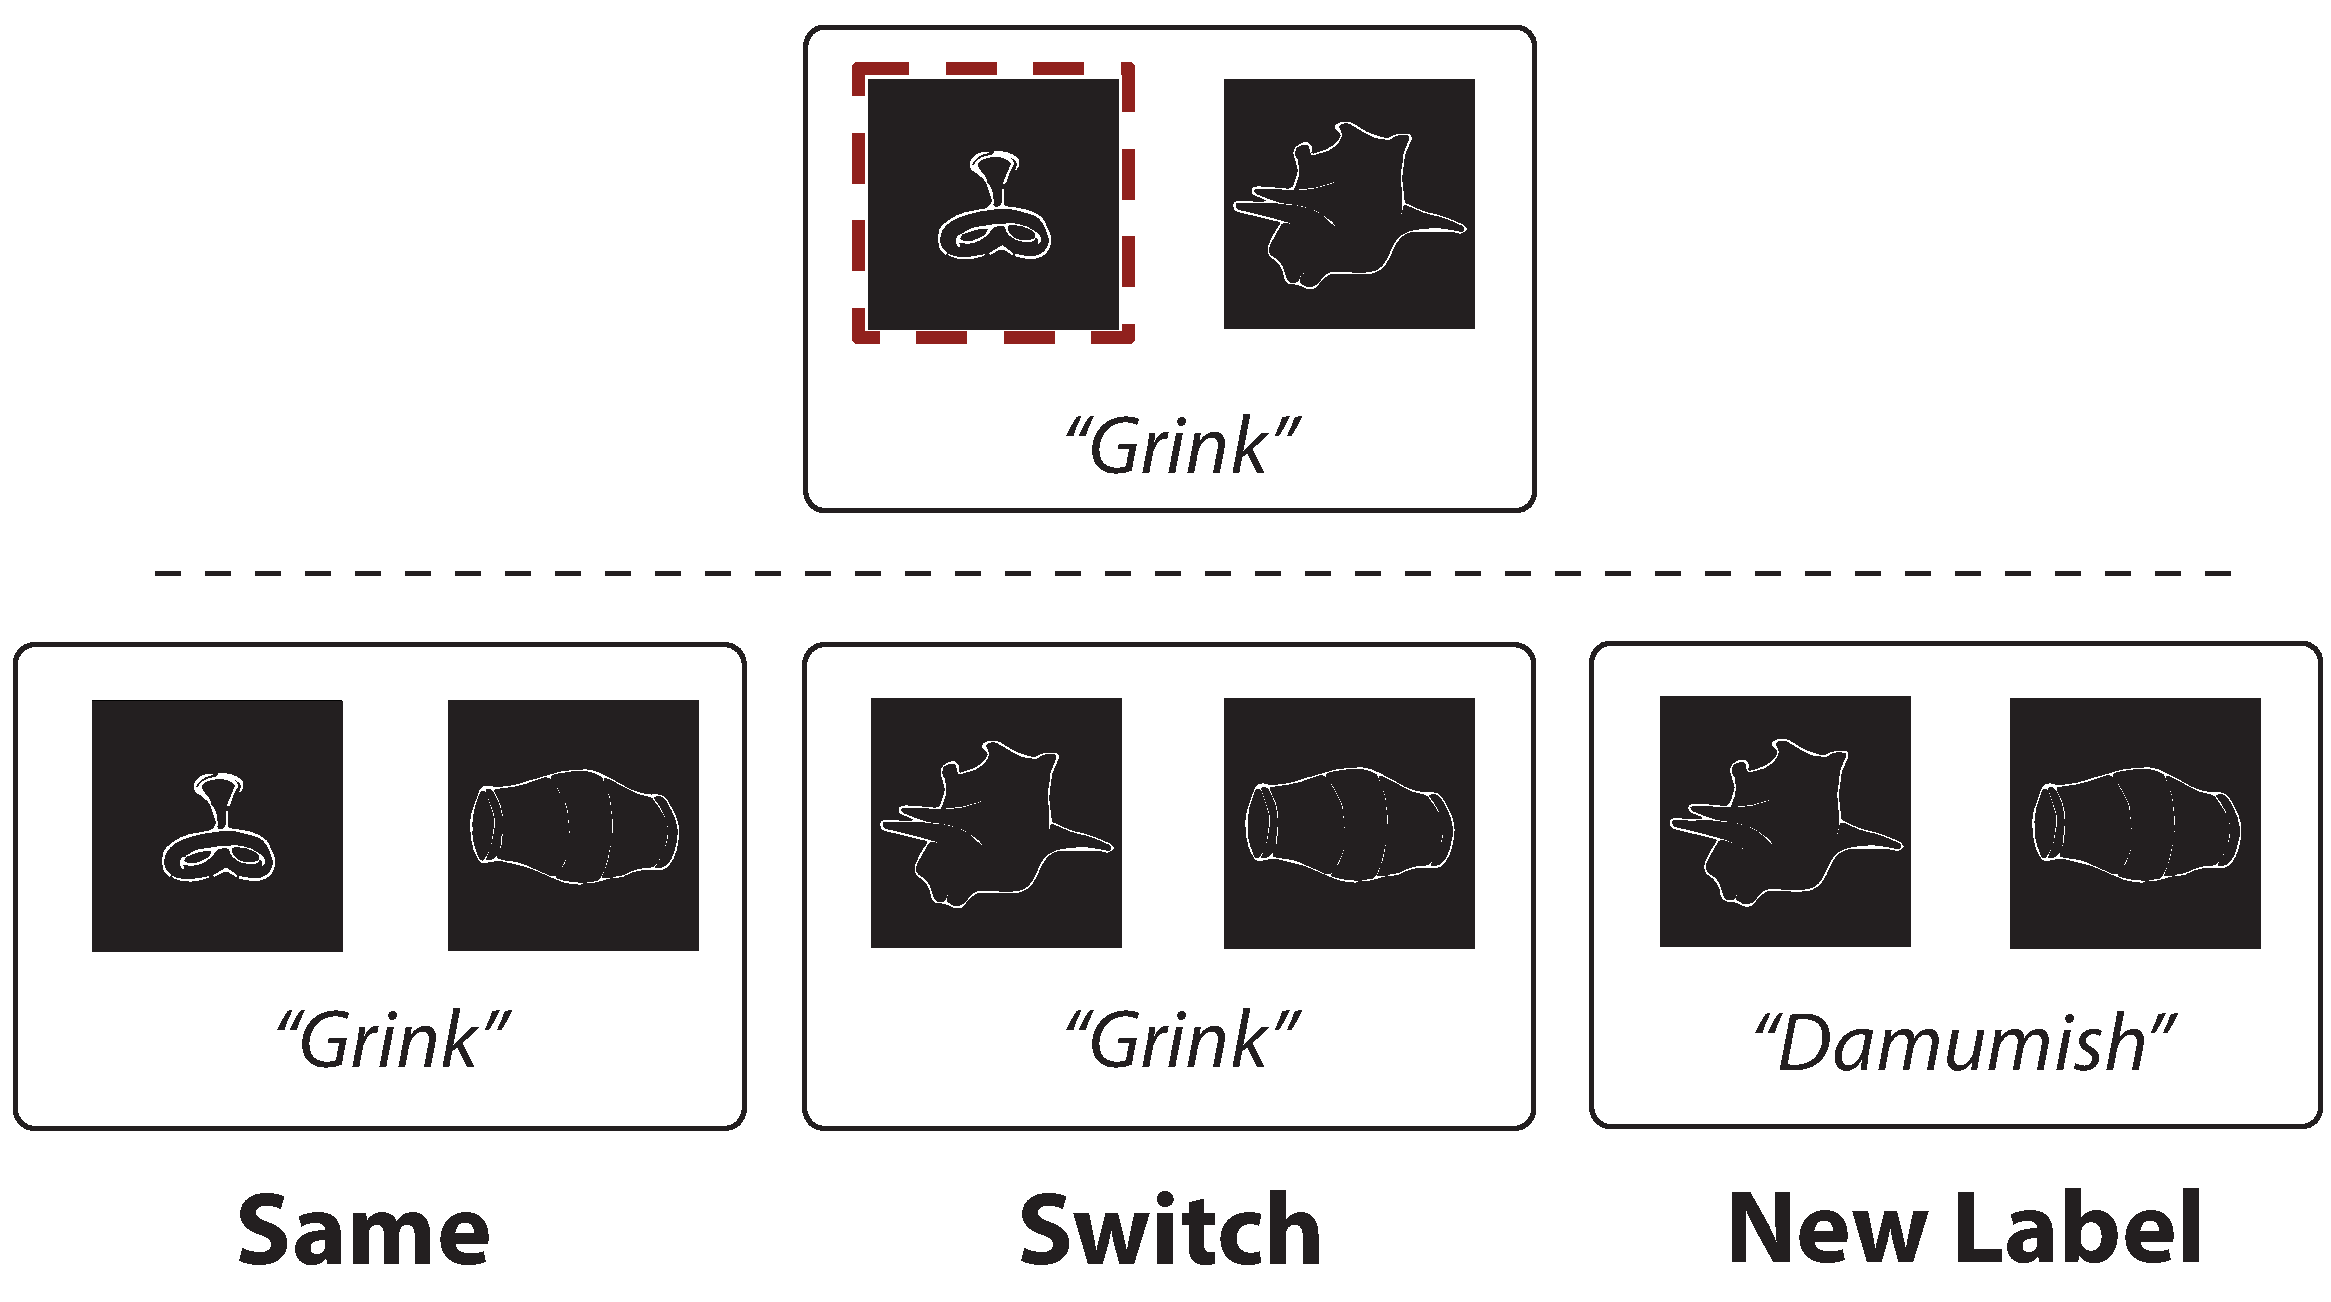
\includegraphics[width=.9\textwidth]{figures/design_fig}}
	\caption{\label{fig:design} A schematic of the experimental trials seen by participants in Experiments 1 and 2. On their first exposure to each novel word, participants were asked to guess its correct referent. In Experiment 1, the second trial for each word was either a Same trial---the set of referents contained the participant's previous hypothesis, or a Switch trial---the set of referents contained one the participant had previously \emph{not} hypothesized. In Experiment 2, Switch trials were replaced with New Label trials that showed same set of referents but a played a novel word. The number of referents on the screen and the interval between successive exposures to the same word varied across conditions.}
\end{figure}

\subsection{Method}

\subsubsection{Participants}

Experiment 1 was posted to Amazon Mechanical Turk as a set of Human Intelligence Tasks (HITs) to be completed only by participants with US IP addresses that paid 30 cents each \cite<for a detailed comparison of laboratory and Mechanical Turk studies see>{Crump2013}. Ninety HITs were posted for each of the 16 Referent x Interval conditions for a total of 1440 paid HITs. If a participant completed the experiment more than once, he or she was paid each time, but only data from the first HIT completion was included in the final data set (excluded 180 HITs). In addition, data was excluded from the final sample if participants did not give correct answers for familiar trials (64 HITs, see Design and Procedure). The final sample thus comprised 1,196 unique participants, approximately 75 participants per condition (range: 71-81).

\subsubsection{Stimuli}

Stimuli for the experiment consisted of black and white pictures of familiar and novel objects and audio recordings of familiar and novel words. Pictures of 32 familiar objects spanning a range of categories (e.g. squirrel, truck, tomato, sweater) were drawn from the set constructed by \citeA{Snodgrass1980}. Pictures of distinct but difficult to name novel objects were drawn from the set of 140 first used in \citeA{Kanwisher1997}. For ease of viewing on participants' monitors, pixel values for all pictures were inverted so that they appeared as white outlines on black backgrounds (see Figure~\ref{fig:design}). Familiar words consisted of the labels for the familiar objects as produced by AT\&T Natural Voices$\texttrademark$ (voice: Crystal). Novel words were 1-3 syllable pseudowords obeying the rules of English phonotactics produced using the same speech synthesizer. 

\subsubsection{Design and Procedure}

Participants were exposed to a series of trials in which they heard a word, saw a number of objects, and were asked to indicate their guess as to which object was the referent of the word. After a written explanation of this procedure, participants were given four practice trials to introduce them to the task. On each of these trials, they heard a Familiar word and saw a line drawing of that object among a set of other familiar objects. On the first two trials, participants were asked to find the squirrel, and the correct answer was in the same position on each trial. On the next two trials, participants were asked to find the sweater, and the correct answer switched positions from the first to the second trial (in order to ensure that participants understood the on-screen position was not an informative cue to the correct target). These trials also served to screen for participants who did not have their audio enabled or who were not attending to the task.

After these Familiar trials, participants were informed that they would now hear novel words, and see novel objects, and that they should continue selecting the correct referent for each word. Participants heard each of the eight novel words twice, but the order in which these words were presented and the number of objects seen on the screen were varied across sixteen between-subjects conditions. Participants saw either 2, 3, 4, or 8 Referents on each trial, and the two trials for each word occurred either back-to-back, or were interleaved between trials for other words for an Interval of 1, 2, 3, or 8. Four of these follow-up trials were Same trials in which the referent that participants selected on the first encounter with that object appeared again amongst the set of objects. The other four were Switch trials in which one of the referents in the set was selected randomly from the objects a participant \emph{did not} select on the previous exposure to that word. All other referents were completely novel on each trial. The number of referents on Familiar trials for each participant matched the number of referents they would see on Same and Switch trials.

Because participants performed this task over the internet, it was important to indicate to them that their click had been registered. Thus, a red dashed box appeared around the object they selected on for 1 second after their click was received. This box appeared around the selected object whether or not it was the ``correct'' referent.\footnote{It is possible that forcing participants to select an object on each trial could have changed their performance. However, control conditions from three previous experiments suggest that empirically this is not the case \cite{Medina2011, Smith2011a, Trueswell2013}.}

\subsection{Results}

Do statistical learners encode multiple referents for each word, or do they instead encode only a single hypothesized referent? The top row of Fig.~\ref{fig:exp1_2_data} shows participants' accuracies in identifying the referent of each word in all conditions for both kinds of trials (Same and Switch). To determine whether participants were learning word-object mappings, we asked whether these accuracies were significantly different than would be expected by chance. Because these accuracies were estimated from a small number of discrete choices for each participant in each condition, they violate the assumptions of standard continuous analyses like $t$ tests. A better model of chance behavior for this data is a $Binomial$ distribution with a probability of success $p=1/\# Referents$. 

 \begin{figure}[tb]
	\center{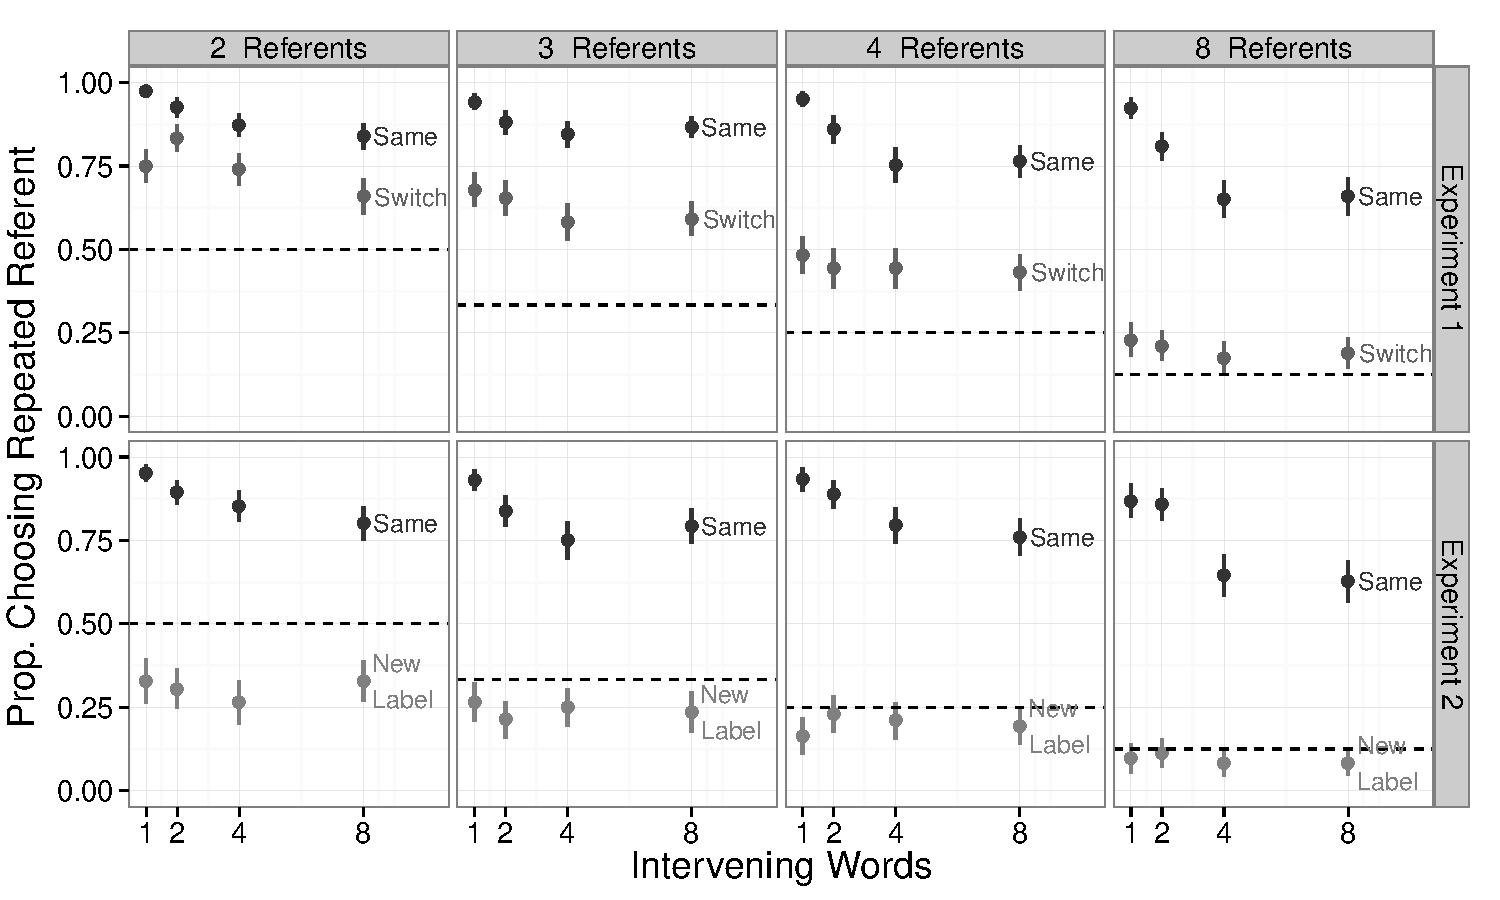
\includegraphics[width=\textwidth]{figures/exp1_2_data}}
	\caption{\label{fig:exp1_2_data} Proportion of repeated referents selected by participants at each combination of number of Referents and Interval on Same and Switch trials in Experiment 1, and Same and New Label trials in Experiment 2. Each datapoint represents $\sim$75 participants in Experiment 1 and  $\sim$50 participants in Experiment 2. Error bars indicate 95\% confidence intervals computed by non-parametric bootstrap. Learning in all conditions of Experiment 1 differed from chance and declined mostly due to Interval for Same trials but mostly due to Referents for Switch trials. Experiment 2 Same trials replicated performance in Experiment 1 Same trials, but New Label trials were different from Switch trials in all Referent and Interval conditions.} 
\end{figure}

To test whether participants' choices were different from those predicted by this null model, we fit we fit logistic regressions for each Referent, Interval, and Trial Type combination. These modes were specified as {\small \tt{Correct $\sim$ 1 + offset(logit($^1/_{Referents}$))}}, where the offset encodes the chance probability of success given the number of referents. The intercept term in each of these models captures on a logit scale how much more likely participants are to select the correct referent than would be expected by chance. At all Referent and Interval levels, both for Same and for Switch trials, participants chose the correct referent more often than would be expected by chance (smallest $\beta =  .393$, $z=2.55$, all $p$s $\leq .01$). Thus, learners encoded more than a single hypothesis in ambiguous word learning situations, even under high levels of memory and attentional load. 

Next, to quantify the effect of each factor on word learning, we fit a mixed-effects logistic regression model to the data from the full dataset \cite{Baayen2008}. All mixed-effects models presented in the paper were implemented in R 3.13 using version 1.1-7 of the \texttt{lme4} package. Because of the complexity of the dataset, we constructed models iteratively, with first main effects and then interaction terms added as long as they significantly improved the fit of the model to the data (measured by likelihood comparison tests using $\chi^2$). In addition, as in the comparison to chance above, we used an offset of $logit$($^1/_{Referents}$) so that each Referents condition was corrected for its different chance performance probability. 

This analysis showed a significant Intercept term---indicating globally above-chance performance---as well as main effects of Interval and Trial Type. In addition, the model showed significant two-way interaction between Referents and Trial Type and Interval and Trial Type (Table~\ref{tab:exp1_reg}). Thus, while word learning was best at low levels of referential ambiguity and at low memory demands, the decreases in word learning observed on Same and Switch trials were due to different factors. For Same trials, the number of Referents played a relatively small role in the difficulty of learning, while the Interval between learning and test played a large role. However, for Switch trials, because performance was comparatively less good at low Intervals, there was relatively little decline in word mapping as Interval increased but a large decline due to number of Referents. 

\begin{table}[tb]
\begin{center}
\begin{tabular}{lrrrrl}
 Predictor & Estimate & Std. Error & $z$ value & $p$ value &  \\ 
  \hline
  Intercept & 4.31 & 0.28 & 15.18 & <.001 & *** \\ 
  Log(Referents) & 0.17 & 0.10 & 1.66 & 0.10 & . \\ 
  Log(Interval) & -0.68 & 0.07 & -9.72 & <.001 & *** \\ 
  Switch Trial & -2.16 & 0.30 & -7.22 & <.001 & *** \\ 
  Log(Referents)*Switch Trial & -0.68 & 0.11 & -6.20 & <.001 & *** \\ 
  Log(Interval)*Switch Trial & 0.54 & 0.07 & 7.34 & <.001 & *** \\ 
   \hline
\end{tabular}\end{center}
\vspace{6pt}
\caption{\label{tab:exp1_reg}Predictor estimates with standard errors and significance information for a logistic mixed-effects model predicting word learning in Experiment 1. The model was specified as \small{\tt{Correct $\sim$ Log(Referents) * TrialType + Log(Interval) * TrialType + offset(logit($^1/_{Referents}$)) + (TrialType | subject)}}.}
\end{table}

These data suggest that neither the single-referent tracking nor the statistical accumulation account of cross-situational word learning is correct. Although learners did encode multiple referents, they did not encode them all with equal strength. Memory for the hypothesized referent was stronger than for non-hypothesized referents at all referent-set sizes and at all intervals. Further, the difference between them grew with number of referents. Thus, it appears that a new account is necessary that integrates elements of both single-referent tracking and accumulative statistical tracking.

Before presenting a formal integrative account in the Model section below, we first rule out one other possibility. Because the set of foils for each target referent was distinct, participants could have succeeded on Switch trials by selecting the most familiar object regardless of which word they were hearing. If so, these data would be consistent with a slightly amended single-referent tracking account in which learners also have some residual memory for previously-seen objects but have not learned them as word-object mappings. Experiment 2 presents a new learning condition to test this possibility.

\section{Experiment 2}

Participants' above-chance accuracies on Switch trials in Experiment 1 provide evidence of their memory for multiple objects, but not necessarily for the formation of referential mappings between the objects and the novel words. To rule out this second possibility, Experiment 2 replaced Switch Trials with New Label trials in which participants saw an object they had previously \emph{not} selected among a set of novel competitors but heard a \emph{New Label} (Fig.~\ref{fig:design}). If success on Switch trials was due purely to referent familiarity, New Label trials should produce similar responses. In contrast, if success on Switch trials was due to a learned mapping between words and referents, New Label trials should show a different pattern of performance.

\subsection{Method}

\subsubsection{Participants}

As in Experiment 1, participants for Experiment 2 were recruited from Amazon Mechanical Turk under the constraint that they had a US IP address. Each HIT paid 30 cents for completion. Sixty HITs were posted for each of the sixteen Referent x Interval conditions for a total of 960 paid HITs. Participants were again paid for multiple HITs, but only data from their first was included in the final set (excluded 100 HITs). In addition, data was again excluded from the final sample if participants did not give correct answers for familiar trials (60 HITs). The final sample thus comprised 803 unique participants, approximately 50 participants per condition (range: 41--55).

\subsubsection{Stimuli, Design, and Procedure}

All aspects of the Stimuli, Design, and Procedure of Experiment 2 were identical to those of Experiment 1 except for the construction of New Label trials. On these trials, the set of candidate referents was the same as on Switch trials in Experiment 1, but the word was novel (Figure~\ref{fig:design}).


\subsection{Results}

Participants showed robust evidence of learning mappings (rather than simply tracking familiar objects). As in Experiment 1, we used logistic regression to determine whether participants chose the previously-seen referent on test trials at above-chance levels. As before, participants selected their perviously guessed referent on Same trials at levels far exceeding chance (smallest $\beta =  1.39$, $z=8.17$, all $p$s $< .001$). In contrast, on New Label trials---in which a novel label was paired with a previously seen but not guessed referent---articipants \emph{never} selected the previous referent at above-chance levels. Further, in the 2 and 3 Referents conditions, they reliably selected the previously seen but not guessed referent at \emph{below} chance levels (largest $\beta =  -.32$, $z=1.95$, all $p$s $\leq .05$). In the 4 and 8 Referents conditions, participants also less frequently than predicted by chance, but this difference was not statistically reliable.

To determine whether performance on these harder New Label trials was nonetheless different from comparable Switch trials in Experiment 1, we again fit an intercept-adjusted a logistic regression for each Referent x Interval condition, but included a Condition (Switch vs. New Label) term: {\small \tt{Correct $\sim$ 1 + Condition + offset(logit($^1/_{Referents}$))}}. The Condition term was reliably different from 0 in all conditions, indicating that participants treated Switch and New Label trials differently (smallest $\beta =  .74$, $z=2.87$, all $p$s $\leq .001$). That is, participants recognized the previous referents on New Label trials from these referents from their first exposure, and further recognized that they did not co-occur on their previous exposure with the label they heard at test (bottom row of Fig.~\ref{fig:exp1_2_data}). This is strong evidence that participants did indeed encode word-object mappings for non-guessed referents even at the highest number of Referents and at the longest Interval.

In addition, a mixed-effects logistic regression largely reproduced the patterns observed in Experiment 1 (Table~\ref{tab:exp2_reg}). Performance on Same trials declined predominantly due to interval, but not due to number of Referents. In contrast, interval had very little effect New Label trials---as was the case for Switch trials in Experiment 1.

\begin{table}[tb]
\begin{center}
\begin{tabular}{lrrrrl}
 Predictor & Estimate & Std. Error & $z$ value & $p$ value &  \\ 
  \hline
  Intercept & 3.42 & 0.21 & 16.10 & <.001 & *** \\ 
  Log(Referents) & 0.32 & 0.06 & 5.52 & <.001 & *** \\ 
  Log(Interval) & -0.60 & 0.07 & -8.22 & <.001 & *** \\ 
  New Label Trial & -4.49 & 0.19 & -23.52 & <.001 & *** \\ 
  Log(Interval)*New Label Trial & 0.58 & 0.08 & 6.89 & <.001 & *** \\ 
   \hline
\end{tabular}
\end{center}
\caption{\label{tab:exp2_reg}Predictor estimates with standard errors and significance information for a logistic mixed-effects model predicting word learning in Experiment 2. The model was specified as {\small \tt{Correct $\sim$ Log(Referents) + Log(Interval) * TrialType + offset(logit($^1/_{Referents}$)) + (TrialType | subject)}}.}
\end{table}

Taken together, these data are strong evidence that neither the single-referent tracking nor the statistical accumulation account of cross-situational word learning is correct.\footnote{One alternative explanation remains possible: Perhaps participants track word and referent familiarity independently, and map familiar words to familiar referents and unfamiliar words to unfamiliar referents, without ever linking the two. For an additional control experiment that rules out this explanation, see the Appendix.} Instead, cross-situational word learning is best characterized by a combination of both of these mechanisms. In the next section, we formalize this idea.

\section{Model}

We begin by describing the computational-level learning problem posed by Experiment 1 using the model developed in \citeA{Frank2009a}. In this framework, the learner observes a set of situations $S$ with the goal of determining the lexicon of word-object mappings $L$ that produced them $P(L|S)$. We can use Bayes' rule to describe the inferential computation the learner must perform: 

\begin{align} 
P(L|S) \propto & \;P(S|L) \: P(L) \label{eq:wurwur1}
\end{align}

\noindent Each situation consists of two observed variables: objects ($O$) and words ($W$). In addition, situations implicitly contain an additional hidden variable: an intention ($I$) by the speaker to refer to one of the objects. Thus, speakers first choose an object from the set and then choose a referential label for it. The probability of a lexicon is given as the joint probability of observing all of the words, objects, and intentions given that lexicon, times the lexicon's prior probability:

\begin{align}
P(L|S) \propto & \prod\limits_{s\in{S}}P(W_{s},I_{s}, O_{s},|L) \: P(L) \label{eq:wurwur2}
\end{align}

\noindent Because the referential intention mediates the relationship between words and objects \cite{Frank2009a}, we can rewrite Equation \ref{eq:wurwur2} using the chain rule:

\begin{align}
P(L|S) \propto & \prod\limits_{s\in{S}}P(W_{s}| I_{s}, L) \: P(I_{s}|O_{s})  \: P(L) \label{eq:wurwur3}
\end{align}

To make predictions from this model, we need to define the probabilities in Eq.~\ref{eq:wurwur3}. Following \citeA{Frank2009a}, we propose that the word ($W$) used to label the intended referent on each trial is chosen uniformly from the set of all words in the lexicon for that object ($L_{o}$). In addition, we propose a simple parsimony prior for the lexicon: A priori, the larger the set of words in the lexicon that refer to the same object $O$, the lower the probability of that lexicon: $P(L_{o}) \propto \frac{1}{|L_{o}|}$. 

We can then take this computational-level description of the problem and add cognitive constraints to understand how the patterns observed in our data arise from the interaction of learning mechanisms, attention, and memory \cite<see e.g.,>{Frank2010a, Shi2010}. We start by describing how participants allocate their attention on each learning trial, a critical point of difference between the two different accounts of cross-situational learning. 

 \begin{figure}[tb]
	\center{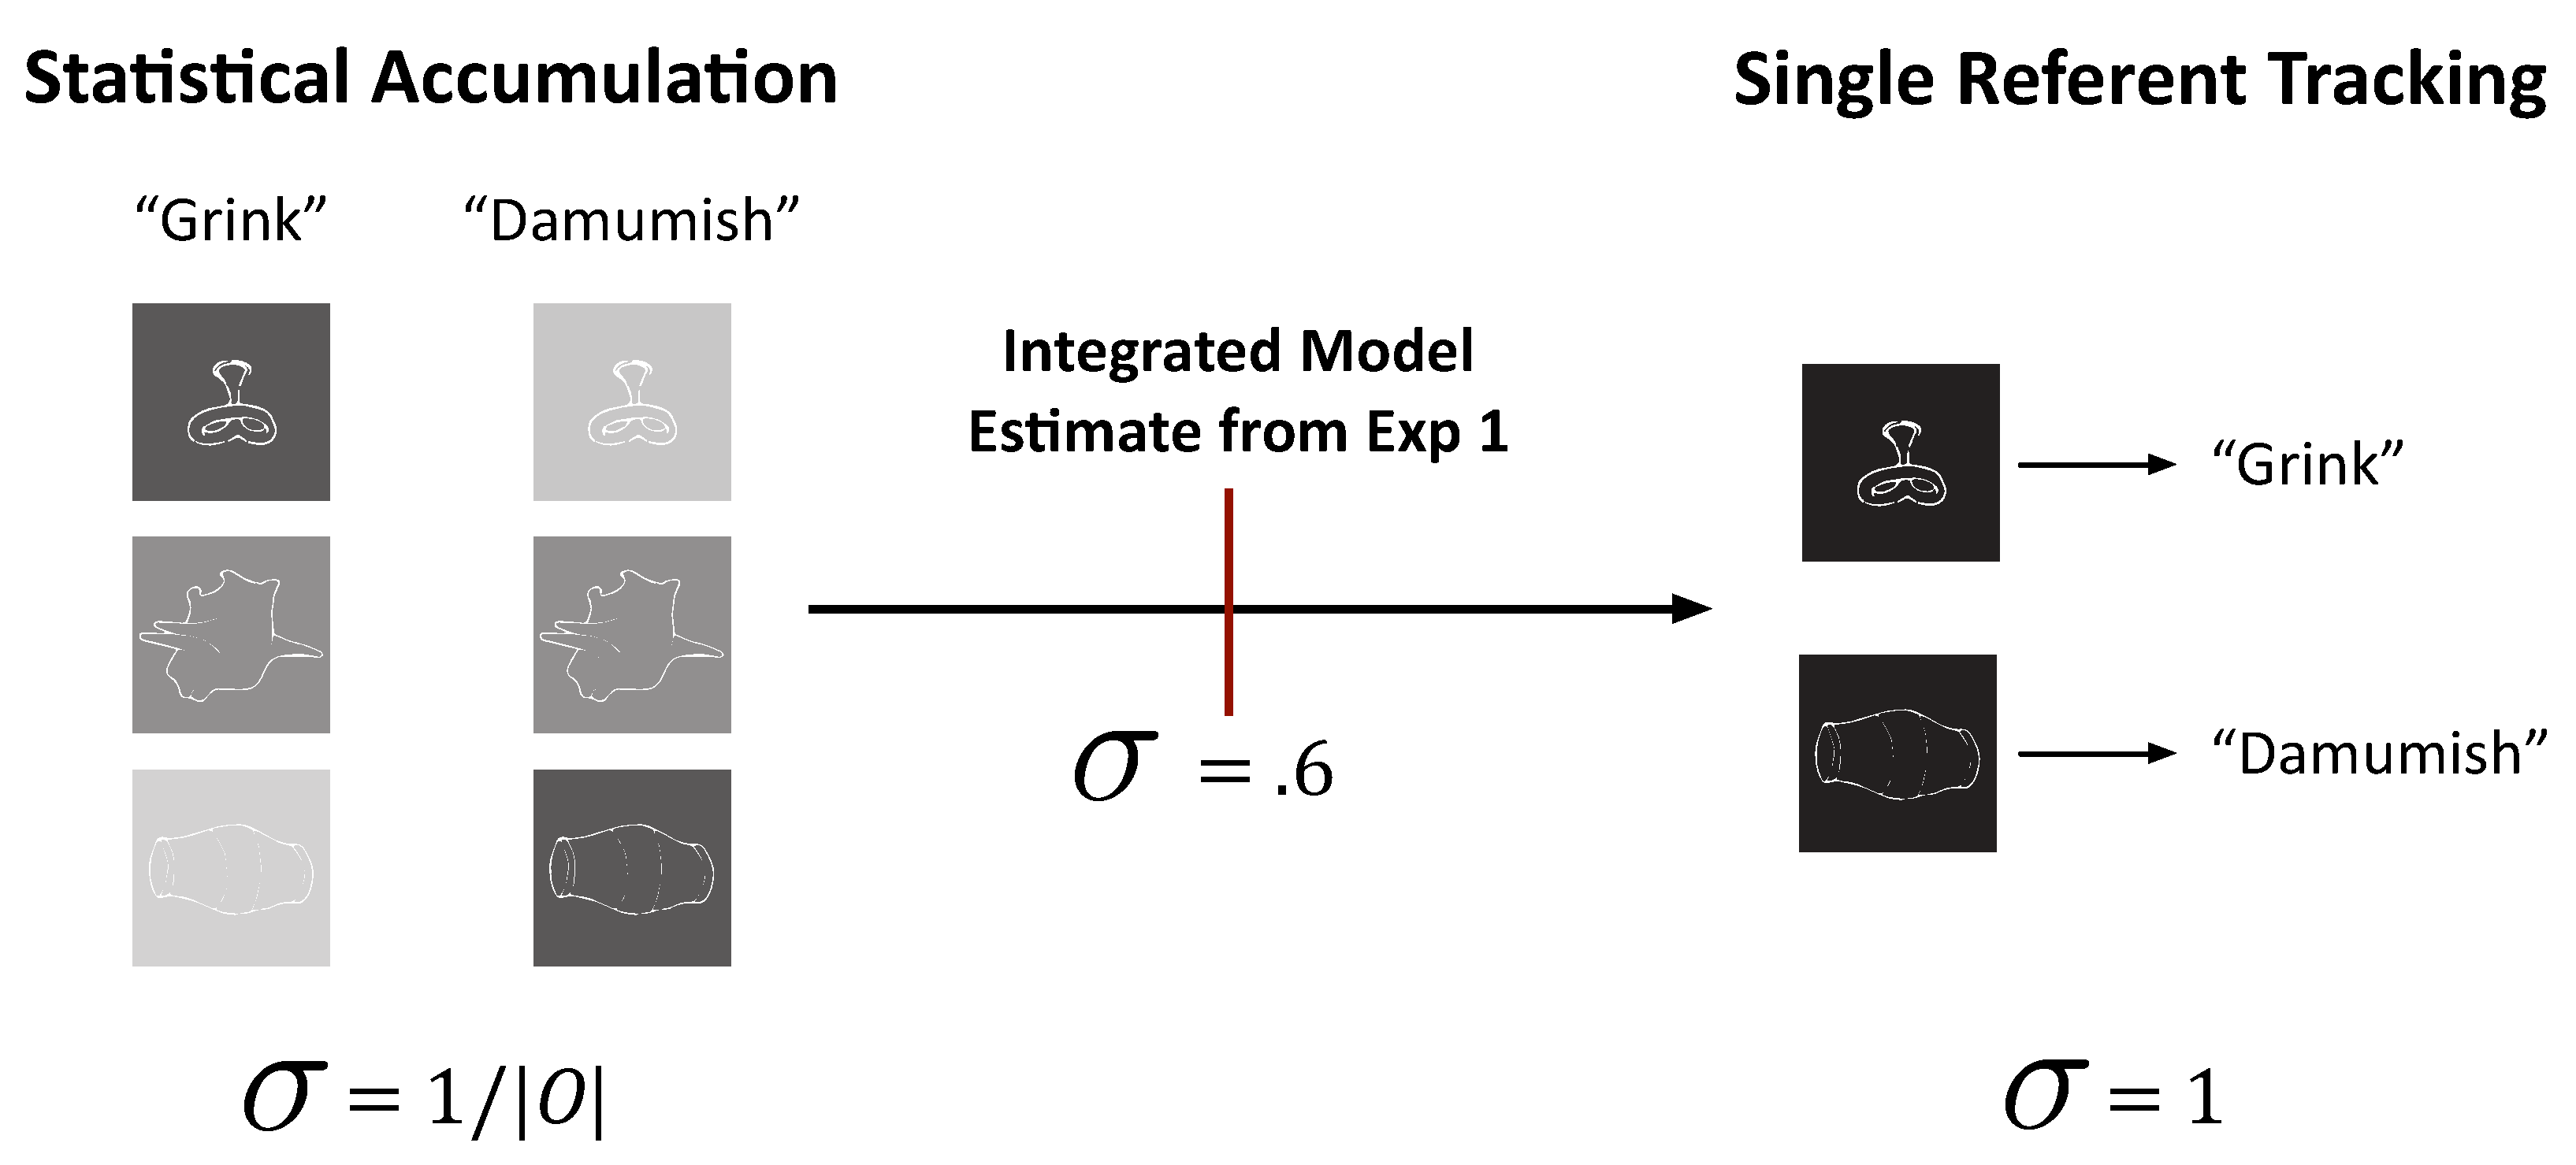
\includegraphics[width=.8\textwidth]{figures/model_fig}}
	\caption{\label{fig:models} A representation of the continuum between the Statistical Accumulation and Single Referent Tracking models as learners' attention is varied from evenly distributed ($\sigma=\frac{1}{|O|}$) to focused on a single referent ($\sigma=1$), as well as the best-fitting integrated model's position along this continuum.}
\end{figure}

In this framework, the most convenient place to integrate attention is in defining the learner's beliefs about $P(I|O)$, the probability of the speaker choosing to refer to each object in the set.\footnote{A full process model should in principle include two distinct components: a learner's inferred beliefs about a speaker's referential intention and the subsequent decision to allocate attention on the basis of these beliefs. But these processes are indistinguishable in our data, and consequently, we collapse them down to a single parameter that controls allocation of attention; future work should distinguish them, however.} One possibility is to let each object be equally likely to be the intended referent, implementing parallel Statistical Accumulation as in \citeA{Frank2009a}. Alternatively, the learner could place all of the probability mass on one hypothesized referent -- implementing a Single Referent tracking strategy. A more flexible alternative is to assign some probability mass $\sigma$ to the hypothesized referent, and divide the remainder evenly among the remaining objects: $\frac{1-\sigma}{|O|-1}$. This Integrated model subsumes the other two as special cases: At $\sigma=1$, it is a Single Referent tracker, and at $\sigma=\frac{1}{|O|}$, it is a parallel Statistical Accumulator (Fig.~\ref{fig:models}).

There is some debate about the mechanisms that give rise to attentional limitations \cite<e.g.>{Wei2012}. In our formulation, attention is treated as a continuous resource, but this choice is a matter of convenience rather than a theoretical commitment. For our purposes, the important question is to what extent attention is focused on the single target referent, and a continuous implementation allows parameter-estimation to answer this question.

Next, we model how learners' memories for observed situations decay over time. We follow previous memory researchers by formalizing memory for a lexical entry as a \emph{power function} of the interval between successive exposures \cite{Anderson1991a}. As with attention-allocation, there a number of successful models of the underlying mechanisms that give rise to phenomena like the power-law observed in human memory \cite<e.g.,>{Murdock1982, Shiffrin1997}. Again, the critical aspect for modeling this data is to be consistent with the broader dynamics of human memory, rather than with determining which model can best account for these dynamics. Accordingly, memory for lexical entry $L_{o}$ decays according to a power function of time $t$ in which $\gamma$ scales the strength of initial encoding and $\lambda$ defines the rate of decay.

\begin{align}
M(L_{o}) = \gamma \, L_{o} \, t^{-\lambda} \label{eq:wurwur4}
\end{align}

Finally, we provide a choice rule describing how learners select among the objects on each test trial. We propose that learners choose the correct referent with probability proportional to their memory for its lexical entry, and otherwise choose randomly among the set of referents (Eq.~\ref{eq:wurwur5}).\footnote{This formulation is equivalent to using Luce's Choice Axiom \cite{Luce1959} with the target having strength  $M(L_{o}) + \frac{1-M(L_{o})}{|O|}$ and each foil having strength $\frac{1-M(L_{o})}{|O|}$.} We use this rule because all of the foils on both Same and Switch trials were novel, and thus should have no trace in memory.

\begin{align}
P(Correct) = M(L_{o}) + \frac{1-M(L_{o})}{|O|} \label{eq:wurwur5}
\end{align}

We implemented our models in R 3.13 using version 2.60 of the \texttt{rstan} package. Raw data for all participants presented in the paper and R code for running the models are available in a github repository at \url{http://github.com/dyurovsky/XSIT-MIN}. All three models---Statistical Accumulation, Single Referent, and Integrated---were fit to the data from Experiment 1 at the individual-participant level. Best-fitting parameters for Experiment 1 for each model were estimated by computing the mean value returned across 1000 samples.

While the Single Referent and Statistical Accumulation models capture some of the structure in the data in Experiment 1, each leaves significant variance unexplained. The Single Referent Model cannot predict above-chance performance on Switch trials, and the Statistical Accumulation model cannot predict a difference between the Same and Switch trials. The Integrated model, however, predicts 95\% of the variance in the data, and significantly outperforms the other models in BIC comparisons as well---a metric that trades off its superior performance against its one additional parameter (Table~\ref{tab:model}). The one mismatch of the model to the data was in switch trial performance for the 3- and 4-referent conditions, in which the integrated model predicted slightly lower performance than that actually exhibited by participants. 

\begin{table}[tb]
\begin{center}
\begin{tabular}{lrrrr}
  Model & Log Likelihood & BIC & E1 $r^{2}$ & E1+2 $r^{2}$ \\ 
  \hline
  Statistical Accumulation & -6565 & 13145 & 0.33 & 0.66 \\ 
  Single Referent & -5950 & 11915 & 0.83 & 0.77 \\ 
  \textbf{Integrated} & \textbf{-5590} & \textbf{11203} & \textbf{0.95} & \textbf{0.97} \\ 
  \hline
\end{tabular}
\end{center}
\caption{\label{tab:model}Likelihood and Correlation measures for models on Experiments 1 and 2. The Integrated model outperformed both of the individual accounts on all measures.}
\end{table}

 \begin{figure}[tb]
	\center{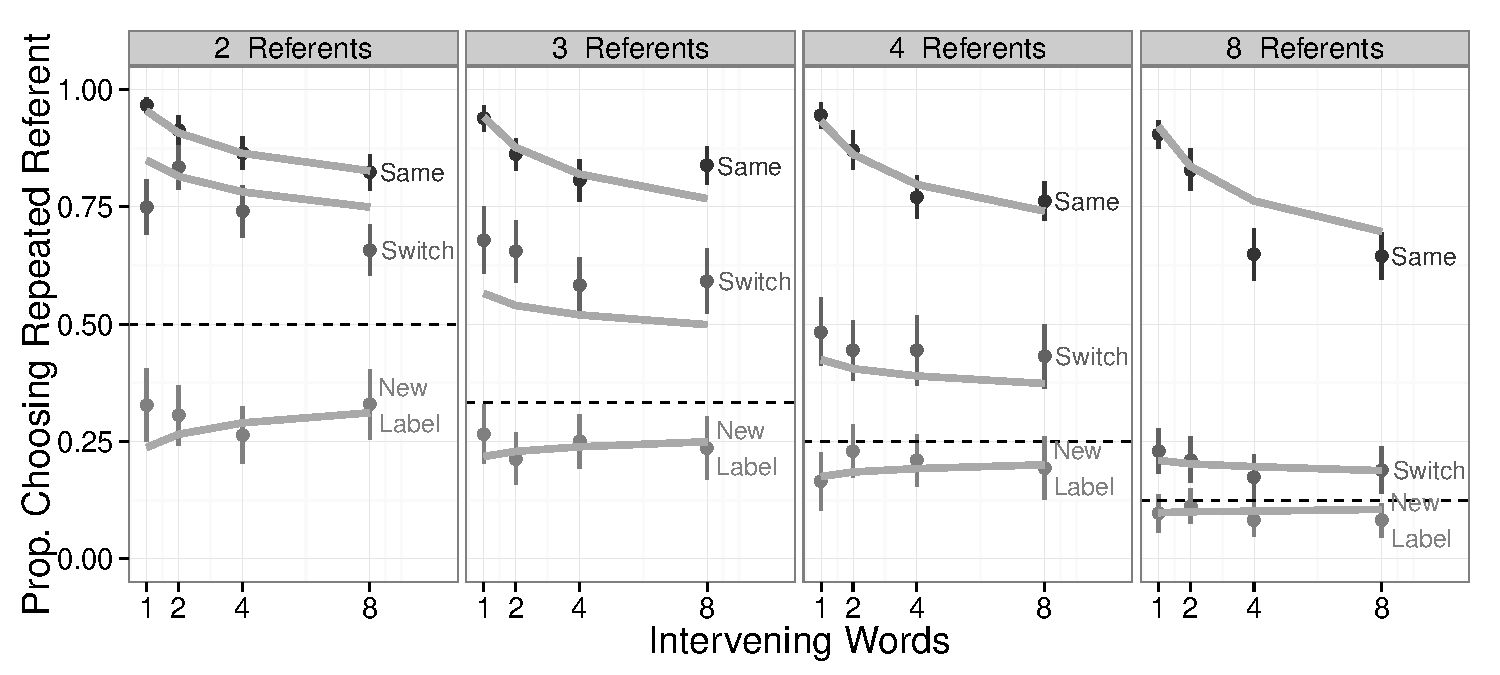
\includegraphics[width=\textwidth]{figures/exp1and2fit}}
	\caption{\label{fig:model_fit} Predictions of the Integrated model for all conditions in Experiment 1 and 2. }
% This model was able to account for 97\% of the variance in the data, significantly outperforming both Single Hypothesis and Parallel Accumulation models.
\end{figure}

We can use the models presented above, with parameters estimated from Experiment 1, to make parameter-free predictions about the data observed in Experiment 2. As before, the Single Referent and Statistical Accumulation models predict some of the variance in the new data, but leave much unexplained. The Integrated model makes near-perfect predictions about the new data---including the New Label condition---explaining 97\% of the combined variance in the data from Experiments 1 and 2 (Table~\ref{tab:model}). Fig.~\ref{fig:model_fit} presents model predictions for all experimental data. Taken together, Experiments 1 and 2 and the integrated model results thus provide strong evidence that learners track not only a single hypothesis for the most likely referent of a novel word, but also some approximation to distributional statistics---in particular, an approximation that becomes less precise as referential uncertainty increases.

\section{General Discussion}

For an ideal learner, word-object co-occurrence statistics contain a wealth of information about meaning. But how is this information used by human learners? One possibility is that learning is fundamentally statistical, and we gradually accumulate distributional information across situations. Another possibility, however, is that we track only a single, discrete hypothesis at any time. While each of these accounts has some support in prior work, neither is consistent with all of the extant data.

Our results here suggest a synthetic explanation: The degree to which learners represent statistical information depends on the complexity of the learning situation. When there are many possibilities, learners represent little about any other than the one that is currently favored; when there are few, learners represent more. This account does not depend on positing multiple, discrete learning systems. Instead, the tradeoff between the most likely hypothesis and the alternatives emerges from graded constraints on memory and attention. Consistent with this account, when we manipulated the cognitive demands of a cross-situational word learning paradigm, we found a gradual shift in the fidelity with which alternatives were represented.

This graded shift in representation was well-described by an ideal learning model, but only when this model was modified to take into account psychological constraints on attention and memory \cite{Kachergis2012,Vlach2013,Yurovsky2014}. This framework allowed us to estimate the effects of these constraints on learning to find the model that best fit the data---one intermediate between the two extreme poles of parallel statistical accumulation and single-referent tracking. This unifying account provides a route by which both hypotheses and sensitivity to statistics can make complementary contributions to word learning \cite{Waxman2009,Kachergis2013}. 

Our account also provides some insight into the conflicting results of previous experiments (Figure~\ref{fig:mrefs}). Because the amount of information participants encode about each non-hypothesized referent falls of proportionally to the number of referents presented, and because the amount of information participants remember falls of proportionally to the interval between successive exposures, statistical power to detect significant information falls of rapidly as the task grows in complexity. Thus, our prediction is that experiments that didn't detect multiple-hypothesis tracking might well have failed because such effects would have been very small and would have required extremely large samples to distinguish such effects from chance with any reliability. And this pattern is further complicated by interactions in the way that participants encode and retrieve information as referents co-occur with multiple different words \cite{Yurovsky2013, Yurovsky2014}. Consequently, we believe that much of the previous confusion has arisen from a combination of measurement and statistical inference issues and a failure to appreciate the effects of particular task parameters on the expected effect size.

The shift from a computational to an algorithmic (or, psychological) description was critical in capturing the pattern of human performance in our task \cite{Marr1982,Frank2010a,Yurovsky2012c}. For the current model, we chose one principled instantiation of cognitive limitations based on previous work, but there may be other consistent proposals. Indeed, the literature contains a number of previous models of cross-situational learning aimed at fitting human-level performance in varying learning conditions with a number of different instantiations of cognitive limitations \cite<e.g.,>{fazly2010,Smith2011a,tilles2013,Kachergis2012,Yurovsky2014}. Problematically, as demonstrated in a recent paper by \citeA{Yu2012b}, these seemingly distinct models can perfectly mimic each other at different parameter settings \cite<see also,>{Townsend1990}. These authors note that modeling choices peripheral to the central learning mechanism---e.g., attentional allocation, memory, choice rule---can be varied to produce many different patterns of learning. 

Our goal in this paper is not to distinguish among competing models, or to ultimately rule them out. Instead, our goal was to be agnostic as possible about the mechanisms underlying cognitive constraints and to ask instead how such constraints produce variation in the fidelity of mapping representations. To facilitate these inferences, we fit a large set of parametrically-varying data that imposes strong constraints on model parameters and modeling choices. In addition, we prevented overfitting by fixing model parameters using Experiment 1 and making parameter-independent predictions about learning that were supported in Experiment 2. This approach allowed us to gain insight about both the central learning mechanism and the constraining processes that together determine human performance.

Although cross-situational learning has been proposed as a potential acquisition mechanism for children \cite<e.g.>{Pinker1989}, the majority of experimental work has focused on adults. While children can learn from cross-situational evidence \cite{Smith2008,Vlach2013,Suanda2014}, the mechanisms underlying these inferences could well be different from those operating in adults. Indeed, some recent findings suggest qualitative differences between children and adults, specifically in scenarios that require exclusion inferences \cite{Ramscar2013}. Any inference from adult data to children's learning mechanisms remains necessarily speculative.

Nonetheless, as more developmental data become available, models like ours will be important tools in interpreting these data. Adults and children differ substantially in general cognitive abilities such as memory and attention \cite<e.g.>{Gathercole2004,Lane1982}. Our model suggests that even if there were continuity in learning \emph{mechanisms} across age, the representations underlying cross-situational learning might still seem to shift between childhood and adulthood. For young children, even ``simple'' two-referent situations might be sufficiently challenging to prevent strong representation of multiple alternatives. Thus, interpretation of new data should be guided by predictions for memory- and attention-constrained learners. 

We further note that connecting experimental data from children to the natural context of word learning may also require substantial work. Cross-situational learning experiments may impose additional cognitive demands on children (e.g., encoding many new words and unfamiliar objects) that are not representative of the familiar circumstances in which children's word learning often takes place. In natural speech to children, referents are introduced into common ground and then discussed \cite{Clark2003}. In contrast, cross-situational tasks are intentionally stripped of the constellation of communicative, attentional, and linguistic cues that typically surround naming events \cite{Frank2013a, Gogate2010, Mintz2003}, and each naming event appears in isolation, rather than being embedded in a coherent discourse \cite{Frank2013a, Rohde2014}. 

Further, while cross-situational learning tasks have typically studied the mapping process independent of the generalization process, children's representations of the meanings of even concrete nouns (e.g. \emph{cup}) appear to follow an extended developmental trajectory, changing well into young-adulthood \cite{ameel2008}. This representational change is likely related both to variability in the examplars children are exposed to, the contexts in which they are seen, and to the other words children have learned and the kinds of hypotheses they have entertained \cite{hidaka2010,Dautriche2014}. Thus, a full understanding of the processes of early word learning will necessarily require further analyses of the natural ecology of word learning and how it changes across development. Nonetheless, data and models of the kind presented here provide useful guiding principles for understanding word learning in the wild.

In sum, our work stands as a case study of how ideal learning models can inform psychological accounts of statistical learning. Although we focused on noun learning, our results are relevant for many problems in language, including phonetic category learning, speech segmentation, and grammar learning. In each of these domains, researchers have debated the degree to which learners represent distributional information \cite{Endress2005, Frank2010a, McMurray2013}. We suggest a synthesis: Learning is fundamentally distributional, but the fidelity of learners' distributional estimates depends critically on their limited attention and memory.

\section{Appendix}

\renewcommand{\thetable}{A\arabic{table}}
\setcounter{table}{0}
\renewcommand{\thefigure}{A\arabic{figure}}
\setcounter{figure}{0}

Experiment 1 showed that participants encode multiple referents in ambiguous naming situations, even under high levels of cognitive load. However, Experiment 1 leaves open the possibility that while participants encoded multiple referents, they did not map them to particular words. Experiment 2 was designed to rule out this unimodal familiarity account, showing that that in the presence of a novel label, participants \emph{dispreferred} the familiar object, suggesting that they encoded words, referents, and something about the relationship between them. However, these results are in-principle consistent with an alternative account in which participants track referent familiarity and word familiarity independently, and use a complex choice rule that selects the most familiar referent in the presence of a familiar word and the most unfamiliar referent in the presence of a novel word. Experiment 3 was designed to test this account.

In Experiments 1 and 2, the set of candidate referents for each word participants learned was distinct from the set of candidate referents for every other word. This experimental choice prevented participants from using knowledge about one word's referent to learn the correct referent of another novel word \cite<c.f.>{Smith2011a,Yurovsky2013}. Choosing to conduct the experiment this way both allowed us to produce better estimates of learning fidelity across conditions and simplified the choice rule necessary for our cognitive model. In Experiment 3, we relax this constraint, however, allowing a more stringent test of the alternative account above. This time, the test set for each word contained both a previously co-occurring (and thus statistically correct) referent, \emph{and} a referent that had been seen more recently, but had co-occurred with a different word. In this way, Experiment 3 directly pitted statistical co-occurrence information against unimodal word and referent familiarity.

\subsection{Method}

\begin{table}[tb]
\begin{center}
\begin{tabular}{| c | c c c | c c c | c c c |}
\multicolumn{1}{c}{ }
 & \multicolumn{3}{c}{Experiment 1}
 & \multicolumn{3}{c}{Experiment 2}
 & \multicolumn{3}{c}{Experiment 3} \\
 \hline
Trial & Word & Ref 1 & Ref 2 & Word & Ref 1 & Ref 2 & Word & Ref 1 & Ref 2 \\ 
\hline
Ex-A& A & a1 & a2 & A & a1 & a2 & A & a1 & a2 \\ 
Ex-B & B & b1 & b2 & B & b1 & b2 & B & b1 & b2 \\ 
T-A & A & a1 & a3 & C & a1 & a3 & A & a1 & b2 \\ 
\hline
\end{tabular}
\end{center}
\vspace{6pt}
\caption{\label{tab:exp3_design}Schematic of the design for Experiment 3. In contrast to Experiments 1 and 2, the test trial (T-A) for each word pitted a previously co-occurring referent (a1) against a more recently exposed familiar competitor referent (b1).}
\end{table}

Table~\ref{tab:exp3_design} shows a design diagram comparing Experiment 3 to Experiments 1 and 2. In Experiment 3, participants again received two trials for each novel word. On the exposure trial (Ex-A), as before, they selected one of the candidate referents. On the test trial for each word (T-A), the set of candidate referents contained one that participants had previously seen on the Exposure trial for that word (a1), \emph{and} one of the referents from the Exposure trial for the intervening word (b2). Our mapping account of the data in Experiments 1 and 2 predicts that participants should select the referent that co-occurred previously with the tested referent (a1). In contrast, a familiarity account of the previous data predicts that participants should select the referent that occurred with the intervening word (b2).

As in the other experiments, we were interested in how learning scales both with the number of referents and with participants' guesses on Exposure trials. We thus tested two referent sizes between subjects: 2 and 4. We also tested all four possible combination of guesses on Exposure trials for the two critical words within-subjects. That is, we compared the referent participants selected on Ex-A to the referent participants selected on Ex-B (Same vs. Same), the referent participants selected on Ex-A to a referent they did not select on Ex-B (Same v. Switch), etc. 

\subsubsection{Participants}

As in Experiments 1 and 2, participants for Experiment 3 were recruited from Amazon Mechanical Turk under the constraint that they had a US IP address. Each HIT paid 30 cents for completion. Because Experiment 3 contained fewer trials per within-subjects condition than experiments 1 and 2, we posted 250 HITs for each Referent condition for a total of 500 paid HITS. Participants were again paid for multiple HITs, but only data from their first was included in the final set (excluded 8 HITs) and additional HIT was posted. In addition, data was again excluded from the final sample if participants did not give correct answers for familiar trials (35 HITs). The final sample thus comprised 465 unique participants, 234 in the 2 Referents condition and 231 in the 4 Referents condition).

\subsubsection{Stimuli, Design, and Procedure}

Experiment 3 used the same Stimuli and general trial structure as Experiments 1 and 2 (Table~\ref{tab:exp3_design}. Each participant received either the 2 Referents or the 4 Referents condition. Each participant was exposed to 8 words, 4 of which were tested and 4 of which provided the Familiar competitors. One of the words was tested in each possible Target vs. Competitor condition (Same v. Same, Same v. Switch, Switch v. Same, Switch v. Switch). In all cases, one Competitor Exposure trial (Ex-B) occurred between the Exposure and Test trials for the Target word, as in the Interval 2 conditions of Experiments 1 and 2. 

\subsection{Results}

Do learners encode mappings for multiple candidate referents, or only do they instead encode words and referents independently? If participants encoded mappings, we would expect them to select the Correct referent more frequently than expected by chance on test trials, even when the Correct referent was one they did not previously select on an Exposure trial. To test this prediction, we again fit adjusted logistic regressions to each condition (\small{\tt{Correct $\sim$ 1 + offset(logit($^1/_{Referents}$))}}). For both 2 and 4 Referents, for all test types, participants selected the Correct referent at levels higher than predicted by chance (smallest $\beta =  .58$, $z=4.25$, all $p$s $< .001$). In the 2 Referent condition, this necessarily means that they chose the Correct referent more frequently than the Familiar referent, as these were the only two options at test. However, in the 4 Referents condition, two other novel competitors were available. To show that participants distinguished between the Correct and Familiar referents in this condition, we need to further show that they were chosen at different rates We thus fit an adjusted logistic regression to determine and asked whether Referent type was a significant predictor of performance (\small{\tt{Correct $\sim$ 1 + Type + offset(logit($^1/_{Referents}$))}}). Indeed, for all test types, the Correct referent was chosen more frequently than the Familiar referent (smallest $\beta =  .61$, $z=3.09$, all $p$s $< .01$). Thus, learners encoded more multiple word-referent mappings, and not just multiple words and referents (Figure~\ref{fig:exp3_data}).

 \begin{figure}[tb]
	\center{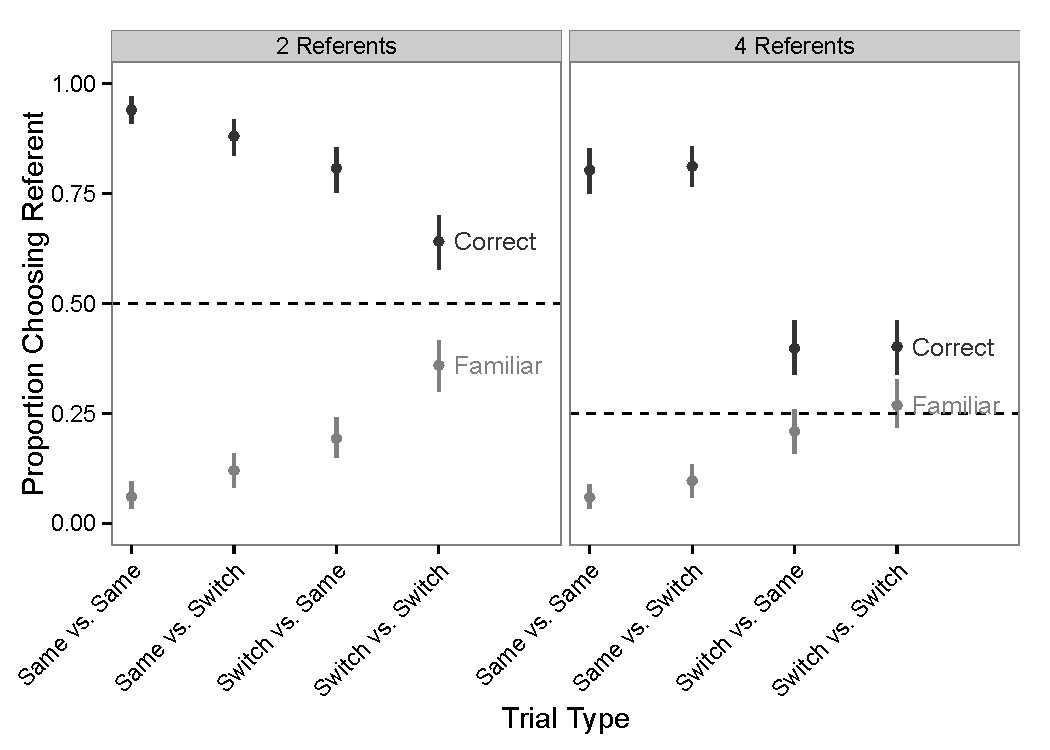
\includegraphics[width=\textwidth]{figures/exp3_data}}
	\caption{\label{fig:exp3_data} Proportion of participants choosing the Correct (co-occurring) and Familiar (most recently seen) referent for each of the four trial types in Experiment 3. Each datapoint represents $\sim$230 participants. Error bars indicate 95\% confidence intervals computed by non-parametric bootstrap. In all cases, participants chose the Correct referent at above chance levels, and also significantly more often than the Familiar referent, indicating that they learned a mapping between words and objects even on Switch trials. Performance decreased predictably when the number of referents increased and when the Correct referent was the one not selected by participants on Exposure trials (\emph{Switch vs. X}).}
\end{figure}

To examine differences across the conditions we tested, we fit a mixed-effects model to determine how performance varied with test type and number of Referents. This model showed a significant Intercept term, indicating globally above-chance selection of Correct referents. It further showed significant main effects Target Type, and Competitor Type, indicating that participants performed best when both the Target and Competitor were referents they had previously hypothesized on Exposure trials. Finally, the model showed significant interaction between both Target and Competitor types and number of Referents, indicating that at 4 Referents the identity of the Target referent had more effect than the identity of the Competitor referent\footnote{Although participants did not receive feedback, one might nonetheless be concerned that because the correct referent in this task was always the referent that was seen two trials ago, participants' above-chance performance on this task might have been due to learning a meta-strategy of selecting the referent from two trials ago. Such an account would predict increased performance over the course of the experiment as participants discovered this strategy. To test this alternative, we added an additional term to the mixed-effects model: Trial number. This regression showed a statistically significant decrease in performance over the course of the experiment (smallest $\beta =  -.132$, $z=-4.93$, $p< .001$), ruling out this account.}. 

In sum, the results of Experiment 3 provide strong support for the account of Experiments 1 and 2 given in the main text: participants in these experiments encoded both their hypothesized referent, and multiple additional referents at above chance levels. Even when the correct referent at test was one that participants had seen but not hypothesized (as in Switch trials in Experiment 1), and even when one of the competitors was seen more recently and thus more familiar, participants selected the correct referent at above chance levels. Further, as in the previous Experiments, performance tracked predictably with both the number of Referents in training and whether the target (and competitor) referent was previously selected by participants on exposure trials. These results thus provide further support for an Integrated model of cross-situational learning in which people encode both a strong single hypothesis and weaker but reliable distributional information about alternative candidate referents. 

\begin{table}[t]
\begin{center}
\begin{tabular}{lrrrrl}
 Predictor & Estimate & Std. Error & $z$ value & $p$ value &  \\ 
  \hline
  Intercept & 3.27 & 0.45 & 7.27 & <.001 & *** \\ 
  Log(Referents) & -0.48 & 0.37 & -1.32 & 0.19 &  \\ 
  Switch Target & -0.92 & 0.42 & -2.17 & 0.03 & * \\ 
  Switch Competitor & -1.77 & 0.40 & -4.40 & <.001 & *** \\ 
  Log(Referents)*Switch Target & -0.75 & 0.36 & -2.07 & 0.04 & * \\ 
  Log(Referents)*Switch Competitor & 1.30 & 0.34 & 3.76 & <.001 & *** \\ 
   \hline
\end{tabular}
\label{tab:exp3_reg}\end{center}
\vspace{6pt}
\caption{\label{tab:exp3_reg}Predictor estimates with standard errors and significance information for a logistic mixed-effects model predicting word learning in Experiment 1. The model was specified as \small{\tt{Correct $\sim$ Log(Referents) * Target + Log(Referents) * Competitor + offset(logit($^1/_{Referents}$)) + (TrialType | subject)}}.}
\end{table}

\bibliographystyle{apacite}
\bibliography{xsit-min}


\end{document}
